\section{High level components and their interaction}
\label{sec:high-level}

The main high level components of the system are the following:
\begin{itemize}
	\item Application server
	\item Web server
	\item Mobile application
	\item Data base
	\item Server side plug-ins:
		\begin{itemize}
		\item ride sharing
		\item ride reservation
		\end{itemize}
	\item User's browser
\end{itemize}

The main components are structured into four layers presented in figure \ref{fig:layers}, which are the following:
\begin {enumerate}
	\item Data base
	\item Application server
	\item Web server
	\item Client
\end{enumerate}

This design choice makes it possible to deploy the application server and the web server on different tiers. It also improves scalability, since there may be many web servers talking to a single application server.

\begin{figure}[h]
\centering
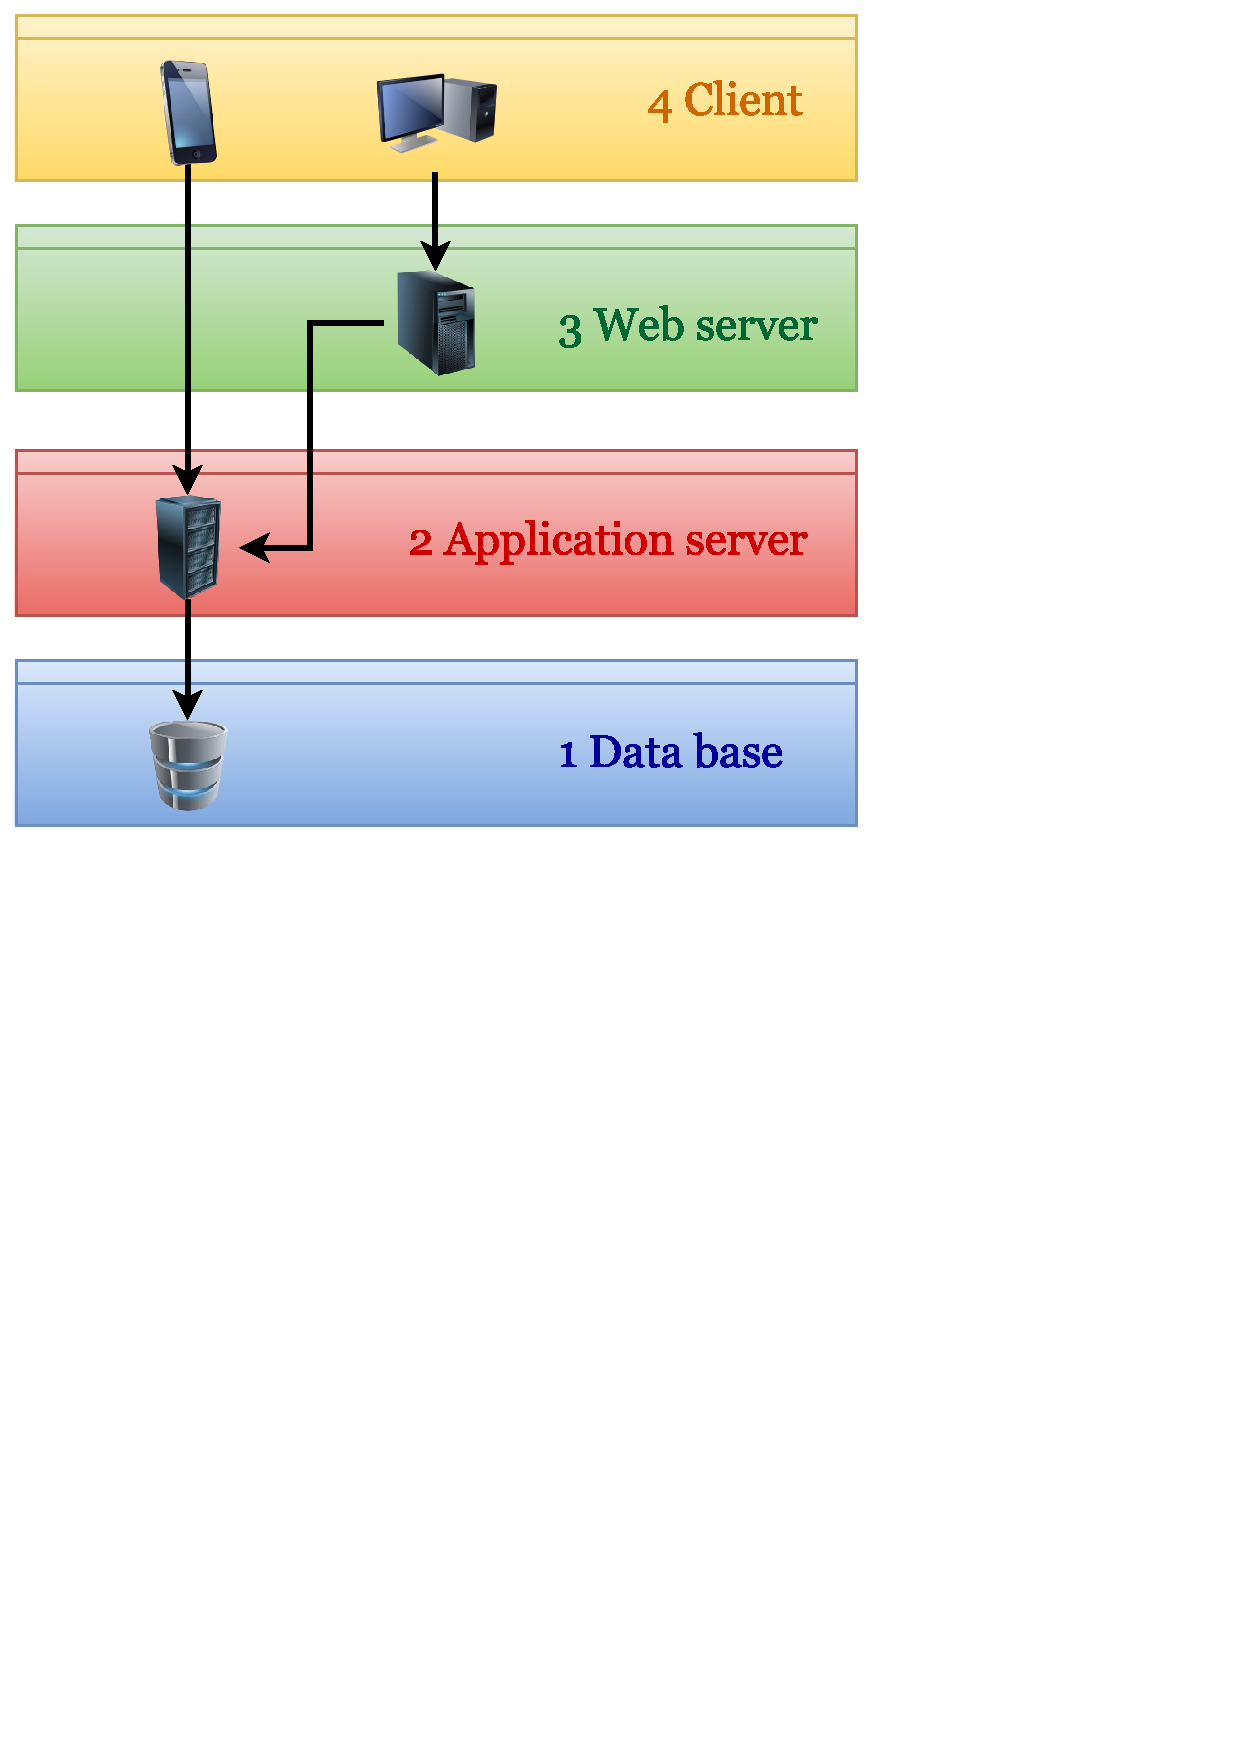
\includegraphics[width=0.7\textwidth]{diagrams/layers.pdf}
\caption{Layers of the system.}
\label{fig:layers}
\end{figure}

The interactions between the main components are shown in the figure \ref{fig:high_level_components} and are asynchronous, except for the interface between the application server and the database, which is synchronous.

\begin{figure}[h]
\centering
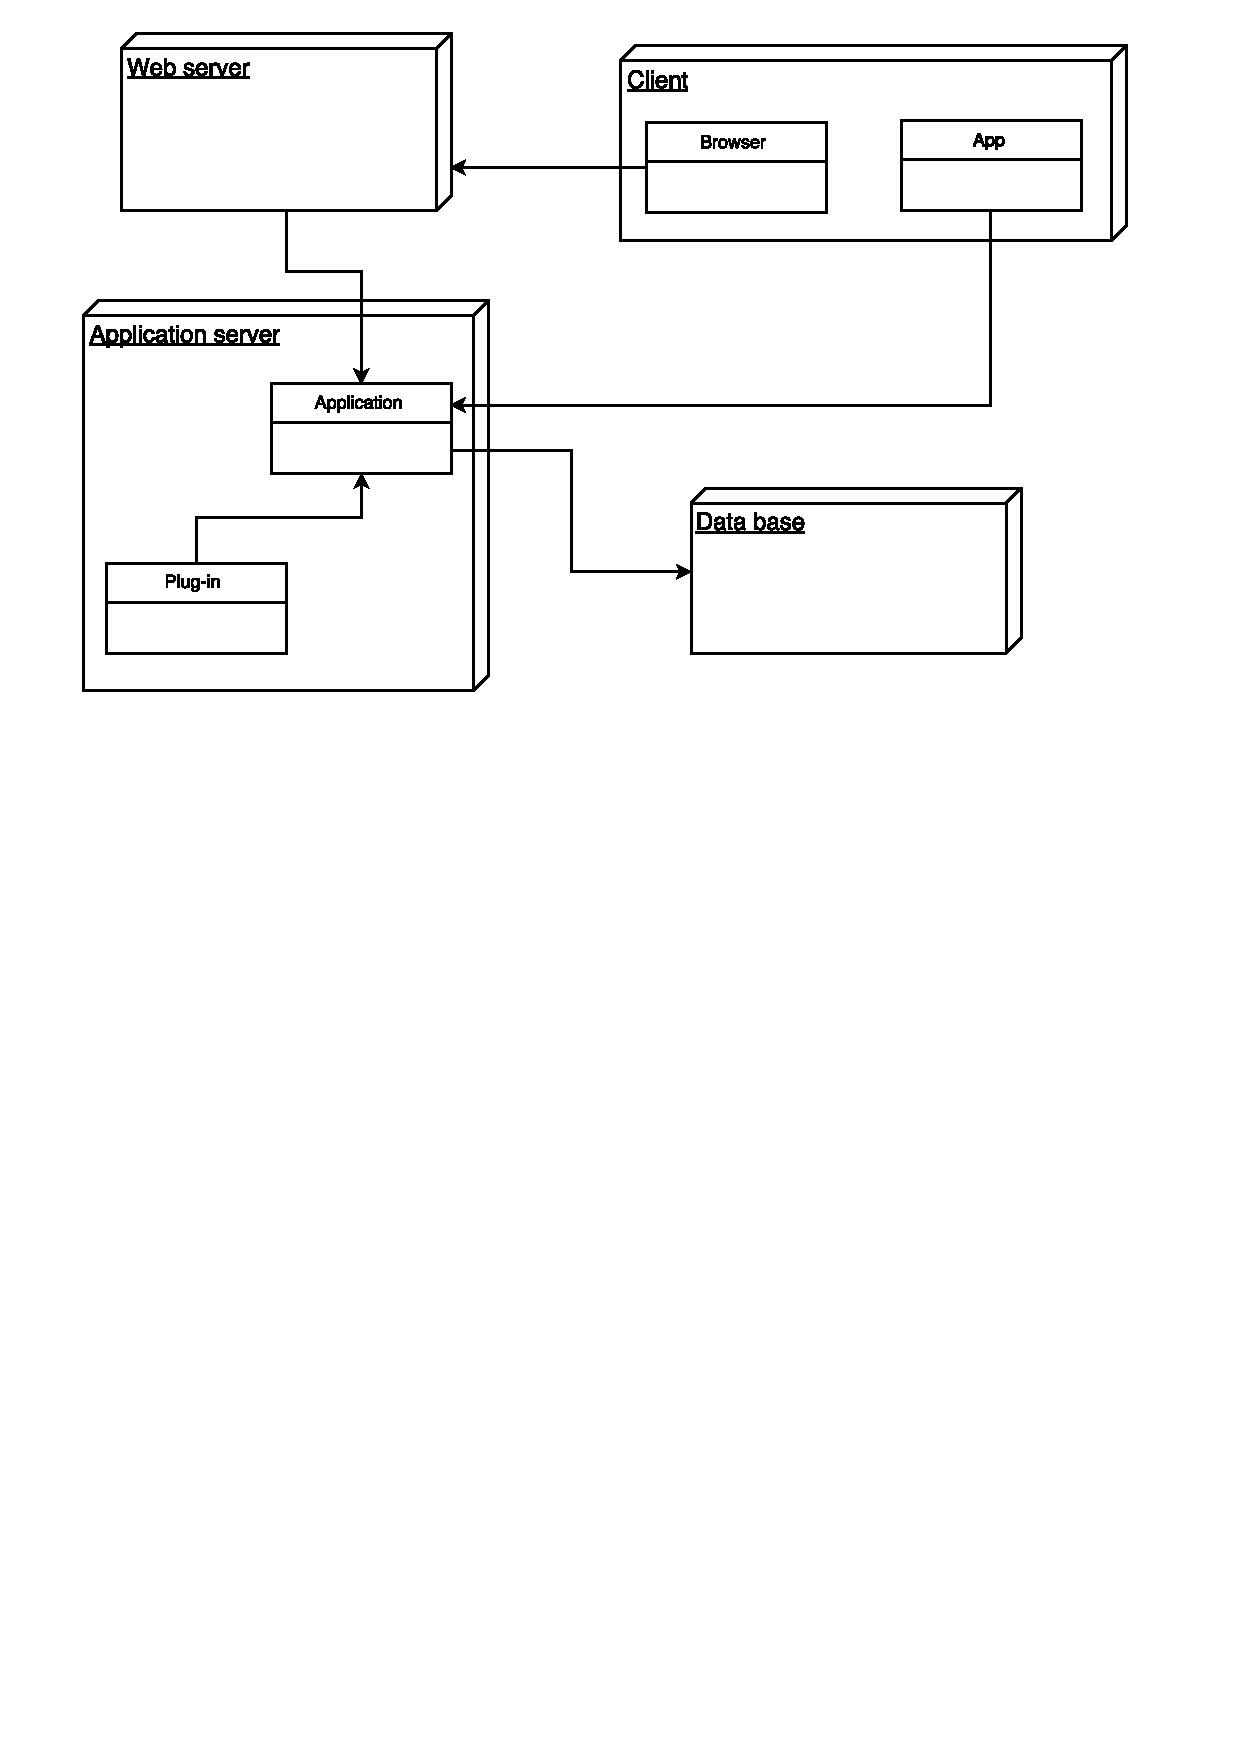
\includegraphics[width=\textwidth]{diagrams/high_level_components.pdf}
\caption{High level components of the system.}
\label{fig:high_level_components}
\end{figure}
